%
% flaeche.tex
%
% (c) 2018 Prof Dr Andreas Müller, Hochschule Rapperswil
%
\documentclass[tikz]{standalone}
\usepackage{times}
\usepackage{amsmath}
\usepackage{txfonts}
\usepackage[utf8]{inputenc}
\usepackage{graphics}
\usepackage{color}
\usepackage{ifthen}
\usetikzlibrary{arrows,intersections,math}
\begin{document}

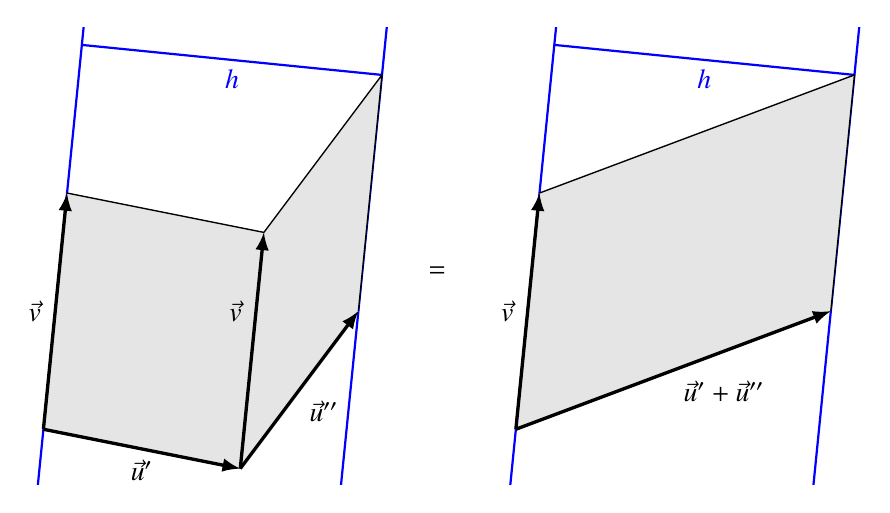
\begin{tikzpicture}[>=latex,thick]

\def\klip{
	\clip (-0.7,-0.7) rectangle (3.9, 5.1);
}

\def\abstand{
	\draw[color=blue] (-0.8,-3)--(0.1,6);
	\draw[color=blue] (3.2,-1.5)--(4.1,7.5);
	\draw[color=blue] (3.8,4.5)--({3.8-3.81188},{4.5+0.38119});
	\node[color=blue] at ({3.8-(0.5*3.81188)},{4.5+(0.5*0.38119)}) [below] {$h$};
}

%\draw (-5,-1) grid (5,6);

\def\O{ (-0.5, 0  )}
\def\v{ ( -0.2, 3  )} % v
\def\u{ ( 2  ,-0.5)} % u'
\def\uu{( 1.5, 2  )} % u''
	\def\uv{(2.3, 2.5)} % u' + v
	\def\U{ (3.5, 1.5)}
\def\vU{(3.8, 4.5)}

\begin{scope}[xshift=-4.5cm]

\klip
\abstand

\fill[color=gray!20] \O--\u--\U--\vU--\uv--\v--cycle;

\draw[line width=0.5pt] \U--\vU--\uv--\v;

\draw[->,line width=1.2pt]  \O--\u;
\draw[->,line width=1.2pt]  \u--\U;
\draw[->,line width=1.2pt]  \O--\v;
\draw[->,line width=1.2pt]  \u--\uv;

\node at (0.75,-0.25) [below] {$\vec{u}'$};
\node at (2.75,0.5) [below right] {$\vec{u}''$};
\node at (-0.4,1.5) [left] {$\vec{v}$};
\node at (2.15,1.5) [left] {$\vec{v}$};

\end{scope}

\node at (0,2) {$=$};

\begin{scope}[xshift=1.5cm]

\klip
\abstand

\fill[color=gray!20] \O--\U--\vU--\v--cycle;

\draw[line width=0.5pt] \U--\vU--\v;

\draw[->,line width=1.2pt] \O--\U;
\draw[->,line width=1.2pt] \O--\v;

\node at (1.5,0.75) [below right] {$\vec{u}' + \vec{u}''$};
\node at (-0.4,1.5) [left] {$\vec{v}$};

\end{scope}

\end{tikzpicture}

\end{document}

